\documentclass[12pt,a4paper]{report}
\usepackage{amsmath}
\usepackage{amsfonts}
\usepackage{amssymb}
\usepackage[german]{babel} %type ngerman if you are using a PC of the university
\usepackage[utf8]{inputenc}
\usepackage{graphicx}
\usepackage[width=150mm,top=25mm,bottom=25mm]{geometry}
%\usepackage{units}
\usepackage{fancyhdr}
\pagestyle{fancy}
\renewcommand{\chaptermark}[1]{\markboth{#1}{}}

\fancyhf{} % clear the headers
\fancyhead[R]{%
   % We want italics
   \itshape
   % The chapter number only if it's greater than 0
   \ifnum\value{chapter}>0 \chaptername\ \thechapter. \fi
   % The chapter title
   \leftmark}
\fancyfoot[C]{\thepage}

\fancypagestyle{plain}{
  \renewcommand{\headrulewidth}{0pt}
  \fancyhf{}
  \fancyfoot[C]{\thepage}
}

\setlength{\headheight}{14.5pt}

%\usepackage{kantlipsum} % for the mock text
\usepackage{enumerate} % enumerados
\usepackage{color}   %May be necessary if you want to color links
\usepackage{hyperref}
\usepackage{setspace}
\usepackage{caption}
\onehalfspacing
\hypersetup{
    colorlinks=false, %set true if you want colored links
    linktoc=all,     %set to all if you want both sections and subsections linked
    linkcolor=blue,  %choose some color if you want links to stand out
	}
\author{Youssef El Mard Bouziani}
\title{Transversalimpulsverteilung geladener Teilchen in Proton-Proton-Kollisionen bei  $\sqrt{s} = 5.02$ TeV in ALICE}
\parindent 0ex

\begin{document}


\begin{titlepage}
\begin{center}

\vspace*{5cm}  

\huge{\textbf{Transversalimpulsverteilung geladener Teilchen in Proton-Proton-Kollisionen bei  $\sqrt{s} = 5.02$ TeV in ALICE}}\\[2cm]
\vfill
\Large{\textbf{Bachelorarbeit}}\\
am Institut für Kernphysik Frankfurt\\
\vfill
vorgelegt von\\[1cm]
\Large{\textbf{Youssef El Mard Bouziani}}\\[1cm]
\vfill
Fachbereich Physik\\
der Goethe-Universität\\
Frankfurt am Main\\

\end{center}
\end{titlepage}
\tableofcontents
\chapter{Einleitung}
\chapter{Physikalische Grundlagen}
\label{cha:PGrundlagen}
\section{Das Standardmodell der Teilchenphysik}
\label{sec:DasSMT}
Das Standardmodell der Teilchenphysik entstand in den 1970er Jahren mit dem Ziel, die Erkenntnisse der Eigenschaften der Elementarteilchen, die die fundamentalen Bausteine der Materie bilden, sowie der \sloppy Wechselwirkungen zwischen ihnen zu beschreiben und zu vereinen. Dieses theoretische Modell umfasst drei fundamentale Wechselwirkungen: die elektromagnetische, die starke und die schwache Wechselwirkung. \\
Alle bisher bekannten Teilchen sind aus kleineren und nach heutigen Wissensstand unteilbaren Elementarteilchen aufgebaut. Alle Teilchen einschließlich der Elementarteilchen lassen sich in zwei Hauptgruppen in Abhängigkeit ihres Eigendrehimpuls, auch Spin genannt, einteilen. Man nennt Teilchen mit halbzahligem Spin Fermionen, während solche mit ganzzahligem Spin als Bosonen bezeichnet werden. Im Standardmodell der Teilchenphysik werden elementare Fermionen in sechs Quarks und sechs Leptonen unterteilt, demgegenüber beobachtet man vier verschiedene Bosonen, die aufgrund ihrer Eigenschaften Austauschteilchen genannt werden. Des Weiteren werden Quarks und Leptonen in drei Generationen bzw. Familien zusammengefasst und man klassifiziert sie simultan in Abhängigkeit ihrer elektrischen Ladung. Teilchen von verschiedenen Familien unterscheiden sich mit Ausnahme von den drei elektrisch neutralen Leptonen, auch Neutrinos bezeichnet, in ihrer Masse. Jedes Fermion einer Generation besitzt eine größere Masse als das Fermion derselben elektrischen Ladung der vorherigen Generation. In der Tabelle \ref{tab:elementareFermionen} sind alle diese Informationen in übersichtlicher Form zusammengefasst. \\
Man unterscheidet, wie bereits erwähnt, sechs Quarks: \textit{up} (\textit{u}), \textit{down} (\textit{d}), \textit{charm} (\textit{c}), \sloppy \textit{strange} (\textit{s}), \textit{top} (\textit{t}) und \textit{bottom} (\textit{b}). Außerdem gibt es zu jedem Quark das entsprechende Antiquark, welches identische Masse aber unter anderem entgegengesetzte elektrische Ladung besitzt. Alle gebundenen Zustände, also Teilchen, die aus Quarks bestehen, werden Hadronen genannt. Wenn ein Hadron aus drei Quarks besteht, bezeichnet man es Baryon. Ist es aber aus einem Quark- und Antiquark-Paar aufgebaut, dann wird es Meson genannt. Zu den bekanntesten Baryonen gehören das Proton \textit{p} (\textit{uud}) und das Neutron \textit{n} (\textit{udd}), welche zusammen alle Atomkerne der bekannten Materie bilden können. \\
Leptonen werden nach ihrer elektrischen Ladung und ihrer Masse eingeteilt. Man sortiert nach den drei elektrisch geladenen Leptonen, das Elektron (\textit{e}), das Myon ($\mu$) und das Tauon ($\tau$), und nach den drei elekrtisch neutalen Leptonen, das Elektron-Neutrino $(\upsilon_{e}$), das Myon-Neutrino ($\upsilon_{\mu}$) und das Tau-Neutrino ($\upsilon_{\tau}$). Die Elektronen bilden zusammen mit den aus Protonen und Neutronen bestehenden Atomkernen alle Elemente, die im Periodensystem der Elemente sortiert sind. Hier sei noch einmal hervorgehoben, dass die alltägliche Materie, die aus Atome besteht, lediglich aus den drei Elementarteilchen der ersten Generation \textit{up}, \textit{down} und Elektron aufgebaut ist. \\
\begin{table}
\centering
\begin{tabular}{|c|c|c|c|c|}
\hline
\multicolumn{1}{|c|}{\textbf{Fermionen}} & \multicolumn{3}{|c|}{\textbf{Generation}} & \multicolumn{1}{|c|}{\textbf{elektrische}} \\
\cline{2-4}
& I & II & III & \textbf{Ladung [e]} \\
\hline
\hline
Quarks & \textit{u} & \textit{c} & \textit{t} & $2/3$\\ 
\cline{2-5}
& \textit{d} & \textit{s} & \textit{b} & $-1/3$\\ 
\hline
\hline
Leptonen & \textit{e} & $\mu$ & $\tau$ & $-1$\\ 
\cline{2-5}
& $\upsilon_{e}$ & $\upsilon_{\mu}$ & $\upsilon_{\tau}$ & $0$\\ 
\hline
\end{tabular}
\caption{Zusammenfassung elementarer Fermionen.}
\label{tab:elementareFermionen}
\end{table} 
\begin{table}
\centering
\begin{tabular}{|c|c|c|}
\hline
\textbf{Wechselwirkung} & \textbf{Austauschteilchen} & \textbf{koppelt an}\\
\hline
\hline
elektromagnetisch & Photon $\gamma$ & Quarks, geladene Leptonen\\
\hline
stark & Gluon \textit{g} & Quarks, Gluonen\\
\hline
schwach & $W^{\pm}$, $Z^{0}$ & Quarks, Leptonen\\
\hline
\end{tabular}
\caption{Fundamentale Wechselwirkungen und dazugehörige Austauschbosonen.}
\label{tab:Wechselwirkungen}
\end{table}
Die Existenz der oben genannten Wechselwirkungen oder Grundkräfte, die man zwischen Elementarteilchen beobachtet, wird in der Theorie durch den Austausch von sogenannten Austauschteilchen erklärt. Es handelt sich um vier Bosonen, die die Grundkräfte vermitteln. In der Tabelle \ref{tab:Wechselwirkungen} findet man eine Übersicht der fundamentalen Grundkräfte. Um genau zu verstehen, wie diese Wechselwirkungen auftreten, muss der Begriff \glqq Ladung\grqq{} verdeutlicht werden. Unter diesem Konzept versteht man in der Teilchenphysik die grundlegende Eigenschaft eines Teilchens, eine bestimmte Wechselwirkung mit einer gewissen Stärke zu erfahren und zu erzeugen. Jede Wechselwirkung hängt also mit einer bestimmten Ladung zusammen. Das massenlose und elektrisch neutrale Austauschboson der elektromagnetischen Wechselwirkung wird Photon ($\gamma$) genannt und koppelt an alle elektrisch geladenen Teilchen. Für die schwache Wechselwirkung sind sowohl die zwei massebehaften, elektrisch geladenen $W^{\pm}$-Bosonen, die jeweils eine entgegengesetzte elektrische Ladung tragen, als auch das massebehafte, elektrisch neutrale $Z^{0}$-Boson verantwortlich. Diese Austauschbosonen koppeln an alle Elementarteilchen. Die starke Wechselwirkung wird hingegen durch das elektrisch neutrale Gluon (\textit{g}) vermittelt, welches nur an Quarks koppeln kann, denn im Unterschied zu Leptonen tragen diese Farbladung, die Ladung der starken Wechselwirkung. Das Gluon selbst trägt ein Farbe-Antifarbe-Paar. Die Farbladung versteht man als den Quantenzustand spezifisch für die starke Wechselwirkung, von dem es drei verschiedene Sorten gibt. Unter Berücksichtigung dieser Aspekte liefern die möglichen Kombinationen zwischen Farbe und Antifarbe zur Bildung eines solchen Paars acht verschiedenen Gluonen. Da für diese Arbeit die starke Wechselwirkung im Besonderen von großer Relevanz ist, wird im folgenden Abschnitt genauer über diese diskutiert und fundamentale Erkenntnisse dargestellt.

\section{Die starke Wechselwirkung}
\label{sec:starkeWW}
%https://web.archive.org/web/20060221233542/http://35.9.69.219/home/modules/pdf_modules/m283.pdf -->Color charge Farbladung
Die Bildung gebundener Zustände aus Quarks lässt sich durch die starke Wechselwirkung erklären. Diese Grundkraft ist dafür verantwortlich, die Quarks anhand ständiges Austauschs von Gluonen zusammenzuhalten. Wie in der Tabelle \ref{tab:Wechselwirkungen} dargestellt ist, koppelt die starke Wechselwirkung nicht nur an Quarks, sondern auch an dem Austauschboson selbst. Die Theorie der starken Wechselwirkung, die Quantenchromodynamik (QCD), befasst sich mit der Beschreibung solcher Phänomene. \\
Die drei verschiedenen Ladungszustände oder Farben, die der starken Kraft zugeordnet werden, werden jeweils in Analogie zur optischen Farblehre \textit{rot}, \textit{blau} und \textit{grün} benannt. Die Antiquarks tragen analog dazu eine Antifarbe. Aus der Mischung der drei Farben oder einer Farbe und der entsprechenden Antifarbe ergibt sich ein farbneutraler Zustand, auch \textit{weiß} genannt. Es konnte durch Experimente gezeigt werden, dass alle Hadronen sich farbneutral verhalten. Dies deutet darauf hin, dass die Quarks eines Baryons jeweils eine verschiedene Farbe tragen, während ein Meson eine Farbe und die entsprechende Antifarbe enthält.\\
Zum besseren Verstehen des Verhaltens der Quarks in gebundenen Zustände muss das Quark-Antiquark-Potential der QCD eingeführt werden, das folgenden Zusammenhang mit dem Abstand $r$ zwischen Quark und Antiquark erfüllt.\\
\begin{equation} \label{eq:PotentialQCD}
  V(r)=-\dfrac{4}{3}\dfrac{\alpha_{s}}{r}+kr
\end{equation}
%Zitat für den Wert der String-Spannung nötig
Dabei bezeichnet $k$ die sogenannte String-Spannung, die einen konstanten Wert aufweist, und $\alpha_{s}$ die Kopplungskonstante der starken Wechselwirkung, die Information über die Stärke der Wechselwirkung liefert. Mit steigendem Abstand $r$ überwiegt der zweite Term $kr$, was ein stark ansteigendes Verhalten des Potentials $V(r)$ verursacht. Dies führt zu einer Verminderung des Verbunds des Quark- und Antiquark-Paars. Wenn man versucht, immer mehr Energie dem Quark-Antiquark-Paar zu zuführen, um es zu trennen, wird die große Energiemenge an einem bestimmten Zeitpunkt ausreichen, um ein neues Quark-Antiquark-Paar zu bilden, das das ursprüngliche Quark und das ursprüngliche Antiquark jeweils in einem gebundenen System behält. In diesem Fall entstehen zwei Mesonen. Die Abbildung \ref{Hadronisierung} stellt schematisch diesen Prozess dar. Das bedeutet, dass ein Quark-Antiquark-Paar sich nicht herauslösen lässt und somit, dass einzelne Quarks nicht beobachtet werden können. Dieses Phänomen bezeichnet man in der Teilchenphysik als \textit{Confinement} (Einschluss). 
\begin{figure}
\centering
\includegraphics[width=5cm]{ErzeugungQuarkAntiquarkPaar.png}  
%Quelle: Elementarteilchen by Christoph Berger
\caption{Hadronisierung durch Energiezufuhr.}
\label{Hadronisierung}
\end{figure}

\begin{figure}
\centering
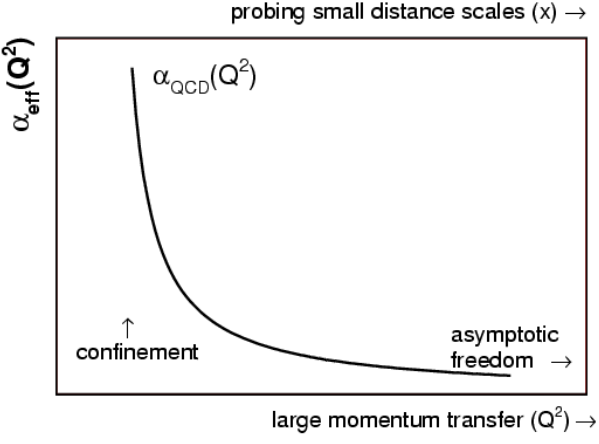
\includegraphics[width=10cm]{KoppKonst.png} 
%Quelle: http://home.thep.lu.se/~torbjorn/talks/durham09.pdf_modules
\caption{Kopplungskonstante der starken Wechselwirkung in Abhängigkeit des Abstands bzw. des Impulsüberträgs.}
\label{KoppKonst}
\end{figure}
Es sollte auch nicht unerwähnt bleiben, wie das Quark-Antiquark-Potential der QCD sich bei kleinen Abständen verhält. In diesem Fall beherrscht der von $1/r$ abhängige Term und damit zeigt das Potential $V(r)$ ein Verhalten ähnlich dem wohlbekannten Coulomb-Potential. Außerdem enthält dieser Term die Kopplungskonstante der starken Wechselwirkung $\alpha_{s}$, die als Funktion des Impulsübertrags $Q^{2}$ wie folgt darstellen lässt:\\
\begin{equation} \label{eq:KoppKonstante}
  \alpha_{s}(Q^{2})\propto\dfrac{1}{\ln{\dfrac{Q^{2}}{\Lambda_{QCD}^{2}}}}
\end{equation}
Dabei bezeichnet $\Lambda_{QCD}$ den sogenannten Skalenparameter der QCD, bei dem $\alpha_{s}$ divergiert. Die Kopplungskonstante $\alpha_{s}$ hängt im Gegensatz zu der Kopplungskonstante der QED sehr stark von dem Impulsübertrag $Q^{2}$ ab. Aufgrund dieses besonderen Merkmales, spricht man von der laufenden Kopplungskonstante (in englisch \textit{running coupling constant}). An dieser Stelle muss man auch besonders betonen, dass kleine Abstände gemäß den aus der De-Broglie-Wellenlänge gezogen Schlussfolgerungen große Impulsüberträge bedeuten. In diesem Zusammenhang ist zu beachten, dass $Q^{2}\propto 1/r$ gilt. Man beobachtet somit, dass die Kopplungskonstante und damit die Stärke der starken Wechselwirkung bei großen Impulsüberträge bzw. bei kleinen Abstände abnimmt und gegen Null geht. Dieser bemerkenswerte Effekt wird asymptotische Freiheit genannt. Das impliziert folgende physikalische Feststellung: Quarks verhalten sich bei sehr hohen Impulsüberträge bzw. bei kleinen Abständen wie quasi-freie Teilchen. Ein solcher Zustand der Materie mit quasi-freien Quarks ist als Quark-Gluon-Plasma (QGP abgekürzt) bekannt. In dieser Arbeit wird eine Messung von Proton-Proton-Kollisionen unter der Annahme untersucht, dass kein solches QGP entsteht. Trotzdem wird das Verständnis des QGP unbedingt benötigt, denn die Messung in dieser Arbeit dient als eine Referenzmessung zu Nukleus-Nukleus-Kollisionen, bei denen tatsächlich ein QGP erzeugt wird. Aus diesem Grund wird im Folgenden auf einige Eigenschaften des QGP eingegangen.
\section{Quark-Gluon-Plasma}
\label{sec:QGP}
\begin{figure}
\centering
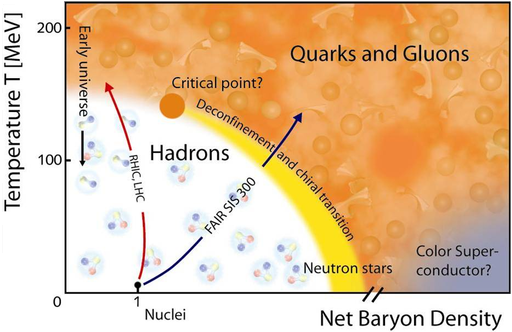
\includegraphics[width=13cm]{Phasenuebergang.png} 
%Quelle: suche sie in Google
\caption{Das Phasendiagramm der Materie. Die Phasen der Kernmaterie sind als Funktion sowohl der Temperatur als auch der Netto-Baryonen-Dichte dargestellt.}
\label{Phasenuebergang}
\end{figure}
Wie im letzten Kapitel erwähnt, können keine freien Quarks beobachtet werden. Allerdings ist heutzutage bekannt, dass das Universum sich während der ersten Augenblicke nach dem Urknall in einem Zustand befand, in dem Quarks aufgrund der hohen Temperaturen keine Hadronen bilden konnten und daher sich wie freie Teilchen verhielten. Dieser Zustand der Materie, in dem Quarks und Gluonen frei existieren ohne gebundene Zustände zu bilden, heißt Quark-Gluon-Plasma. \\
Um ein umfassenderes Verständnis des QGP zu bekommen, muss der Phasenübergang von hadronischer Materie zum QGP untersucht werden. Die Abbildung \ref{Phasenuebergang} zeigt ein Phasendiagramm, das die zwei unterschiedlichen Phasen der Kernmaterie in Abhängigkeit von zwei Zustandsgrößen, der Temperatur und der Netto-Baryonen-Dichte darstellt, die das Verhältnis von Materie und Antimaterie beschreibt. Dazu ist anzumerken, dass die gelbe Kurve, die die jeweils in Weiß und in Orange gekennzeichneten Zustände voneinander abgrenzt, zurzeit nur vermutet werden kann. Nach unserem aktuellen Verständnis der Kernmaterie ist dann zu erwarten, dass man zum QGP auf die beiden Extremen kommen kann: entweder durch Erreichung einer hohen Temperatur oder bei sehr hohen Baryonen-Dichten. Enorm hohe Temperaturen wie im frühen Universum führen zu hohen Energien, was sich in der Ausbildung des QGP niederschlägt. Demgegenüber wohnen Baryonen bei einer hohen Dichte, äquivalent zu hohem Druck, so eng zusammen, dass sie sich überlappen, bis man sie voneinander nicht mehr unterscheiden kann. Aus diesem Phänomen entsteht ebenso ein QGP. In der Natur könnte sich ein Beispiel für dieses Szenario in den Zentren von Neutronensternen finden.\\
Angesichts dessen wird die Untersuchung des QGP sowie seiner Eigenschaften absolut notwendig, um unsere Erkenntnisse über die Struktur der Kernmaterie weiter zu vertiefen. Dafür muss man die Bedingungen zur Ausbildung eines QGP auf der Erde reproduzieren. Zu diesem Zweck setzt man sogenannte Schwerionenbeschleuniger, wie beispielsweise den LHC\footnote{\textit{englisch: Large Hadron Collider}}, ein. In einer solchen anspruchsvollen Anlage werden hochrelativisisch beschleunigte Schwerionen zur Kollision gebracht. Dadurch kann genügend Energie zur Erzeugung eines QGP bei einer niedrigen Netto-Baryonen-Dichte erreicht werden. Aus diesen ultrarelativistischen Schwerionenkollisionen entsteht eine breite Anzahl von Teilchen, die mit Hilfe von Detektoren entsprechend gemessen werden. Daraus lassen sich vielfältige Rückschlüsse über das QGP ziehen, die unseren Blick auf die Teilchenphysik vertiefen.

\section{Monte-Carlo-Simulationen}
\label{sec:MC}
Um die Faktoren zu minimieren, die auf die gemessenen Daten eines hochenergetischen Experiments auswirken und die dadurch die Abweichung dieser Messdaten verursachen, müssen Korrekturen anhand computergesteuerter Simulationen angewendet werden. Diese Simulationen müssen in der Lage sein, die identischen Bedingungen des Experiments zu reproduzieren und die daraus resultierenden Ergebnisse auszuwerten. Diese Situation wirft allerdings folgendes Problem auf: die erwähnten Simulationen müssen sich exakt an die von dem QCD vorgeschlagenen Modellen anpassen, die analytisch nicht gelöst werden können oder die aufwendige numerische Lösungen fordern. Aus diesem Grund verwendet man zur Erzeugung der Simulationen eine probabilistische und hocheffektive Methode, die sogenannte Monte-Carlo-Studie.\\ 
Die Monte-Carlo-Studie basiert auf der Beobachtung, dass die relative Häufigkeit eines Zufallsergebnisses an die theoretische Wahrscheinlichkeit dieses selben Zufallsergebnisses annähert, wenn man das Zufallsexperiments oft genug unter denselben Bedingungen widerholt. In der Teilchenphysik lassen sich Teilchenkollisionen mithilfe einer computergestützten Monte-Carlo-Studie gemäß der QCD nachbilden. Anschließend werden entsprechend Zufallswerte ausreichend häufig erzeugt, um das Verhalten der aus der Kollision resultierenden Teilchen zu ermitteln, wie z.B. die eingeschlagenen Zerfallsketten oder die kinematischen Eigenschaften der Teilchen. Es sei jedoch vermerkt, dass man am Ende kein eindeutiges Ergebnis erhält, sondern eine Wahrscheinlichkeitsverteilung. Solche Monte-Carlo-Studien, die für die Beschreibung von Prozesse in der QCD gebraucht werden, sind als Monte-Carlo-Simulationen bekannt.\\
%WICHTIG: zu korrigieren: GEANT3->Detector, PYTHIA6->Event Genarator
In der Hochenergiephysik werden die Programme, die Monte-Carlo-Simulationen durcführen, Monte-Carlo-Generatoren bezeichnet. Im vorliegenden Fall wird der Monte-Carlo-Generator GEANT3\footnote{englisch: \textit{\textbf{GE}ometry \textbf{AN}d \textbf{T}racking}} zur Korrektur der Messdaten verwendet, welcher den Durchgang elementarer Teilchen durch Detektoren simulieren kann. Außerdem besitzt GEANT3 im Unterschied zu anderen Monte-Carlo-Generatoren die Fähigkeit, das Ansprechverhalten der Detektoren zu beschreiben.
%http://lambda.phys.tohoku.ac.jp/~kobayash/seminar/files/cern/geant.pdf
%https://arxiv.org/pdf/0710.3820.pdf
\chapter{Experimenteller Aufbau}
\label{cha:EAufbau}
Die Durchführung der erwähnten experimentellen Messungen und damit die Forschung der Struktur der Materie werden im Europa durch die Europäische Organisation für Kernforschung (CERN\footnote{französisch: \textit{\textbf{C}onseil \textbf{E}uropéen pour la \textbf{R}echerche \textbf{N}ucléaire}}) ermöglicht. Dieses ambitioniertes Projekt hat seinen Sitz in Genf und entwickelt sich derzeit dank der Beteiligung von 22 europäischen Mitgliedstaaten. Im Rahmen dieser Zusammenarbeit sind vier große Experimente eingerichtet: ATLAS\footnote{englisch: \textit{\textbf{A} \textbf{T}oroidal \textbf{L}HC \textbf{A}pparatu\textbf{S}}}, CMS\footnote{\textit{\textbf{C}ompact \textbf{M}uon \textbf{S}olenoid}}, ALICE\footnote{\textit{\textbf{A} \textbf{L}arge \textbf{I}on \textbf{C}ollider \textbf{E}xperiment}} und LHCb\footnote{\textit{\textbf{L}arge \textbf{H}adron \textbf{C}ollider \textbf{b}eauty}}. Das CERN beherbergt der größte Teilchenbeschleuniger der Welt, der LHC, und wird somit weltweit führend bei der wissenschaftlichen Recherche.  
\section{LHC}
\label{sec:LHC}
Im Jahr 2008 wurde der zur Zeit leistungsstärkste Teilchenbeschleuniger LHC erstmals in Betrieb gesetzt. Diese ringförmige Einrichtung, deren Umfang $26.7$ km beträgt, gehört zum Typ von Teilchenbeschleunigern Synchrotron und ist daher in der Lage zwei beschleunigte Teilchenstrahlen auf kreisförmige Bahnen zu halten. Die Teilchenstrahlen erreichen annähernd Lichtgeschwindigkeit und bewegen sich in entgegengesetzten Richtung durch Ultrahochvakuum, bis sie kollidieren. Damit sie die festgelegten Kreisbahnen perfekt beschreiben, verwendet man supraleitende Elektromagneten, die über ständige Helium-Versorgung zur Abkühlung auf eine Temperatur kleiner als $2$ K verfügen. Die durch diese Magneten erzeugte Feldstärke bestimmt die maximale erreichbare Energie.
\section{ALICE}
\label{sec:ALICE}
ALICE
\subsection{Inner Tracking System}
\subsection{Time Projection Chamber}
%Explicar les paraules: end plates (Endplatte), row (Reihe) i cluster (Cluster)

\chapter{Analyse}
\label{chap:Analyse}
Die Gesamtenergie der Protonen, die kollidieren, ergibt sich aus der Addition der Ruhenergie und der kintetischen Energie dieser Teilchen. In der Teilchenphysik ist sie als Schwerpunktsenergie $\sqrt{s}$ bekannt und stellt eine entscheidende Größe bei der Berechnung von Streuprozessen dar. Zur Untersuchung von Stoßvorgänge berücksichtigt man ferner den zur Strahlachse senkrecht stehenden Impulsanteil, den Transversalimpuls $p_{\mathrm{T}}$. Dieser transversale Impulsanteil kann nur durch eine Kollision entstehen. Andernfalls besitzen Teilchen auf Grund der Beschleunigung im LHC nur einen longitudinalen Impulsanteil. \\
Diese Arbeit untersucht Proton-Proton-Kollisionen bei einer Schwerpunktsenergie $\sqrt{s} = 5.02$ TeV, die mit dem ALICE-Detektor gemessen wurden. Dabei werden hier nur die erzeugten geladenen Teilchen betrachtet. Die gemessenen Daten werden anschließend verarbeitet, um eine Verteilung des Transversalimpulses oder $p_{\mathrm{T}}$-Spektrum zu erhalten. Das $p_{\mathrm{T}}$-Spektrum wird dann mit Ergebnissen, die anhand von MC Simulationen gewonnen wurden, verglichen und durch Verwendung verschiedener Strategien, die im folgenden Abschnitt ausführlich dargestellt werden, entsprechend korrigiert. Schließlich wird der Einfluss der systematischen Unsicherheiten auf das korrigierte $p_{\mathrm{T}}$-Spektrum untersucht.
\section{Datenauswahl}
Im ALICE werden die erfassten Daten gemäß dem Jahr, in dem ihre Messung vorgenommen wurde, eingeteilt. Eine solche jährliche Datennahme besteht aus Messintervalle oder Perioden, die ungefähr ein Monat umfassen. Zur Bezeichnung einer konkreten Periode benutzt man folgende Notation: LHC\{Jahr\}\{Kleinbuchstabe\}. Die kleinste Einheit der Datennahme heißt \textit{run}. Man fasst \textit{runs}, welche mit einer Ziffer kennzeichnet werden, zu Perioden zusammen.\\
In dieser Arbeit werden gemessene Daten, die aus den Perioden LHC17pq stammen, betrachtet. Diese Perioden unterteilen sich in zwei Datenmengen in Abhängigkeit davon, ob die gemessenen Ereignisse mithilfe der SDD-Schichten des ITS rekonstruiert wurden oder nicht. Der Grund, warum man entscheidet, ob der SDD zur Rekonstruktion zu verwenden ist, liegt an folgendem Phänomen dieses Teilchendetektors. Nachdem ein Teilchen mit diesem Detektor gemessen wird, vergeht eine Zeitspanne aufgrund technischer Merkmale, während der kein weiteres Teilchen nachgewiesen werden kann. Diese Zeitspanne nennt man Totzeit. Für die SDD-Schichten dauert sie im Vergleich zum restlichen Detektor sehr lang. Dies bedeutet, dass man durch Verzicht auf den Einsatz der SDD-Schichten viel Zeit sparen kann und dadurch viel mehr Kollisionen messen kann, indem man allerdings Präzision opfert. Die Datenmenge, die die ohne SDD-Schichten rekonstruierten Ereignisse enthält, benennt man \textit{FAST}, während die gemessenen Ereignisse der anderen Datenmenge, die unter dem Namen \textit{CENT} bekannt ist, hingegen mittels der SDD-Schichten festgelegt wurden. \textit{CENT} geht aber noch einen Schritt weiter, indem sie die selben Ereignisse ein zweites Mal ohne die SDD-Schichten rekonstruiert. Diese Tatsache erleichtert den Vergleich zwischen mit und ohne SDD rekonstruierten Ereignisse. In der Tabelle \ref{tab:CENTundFAST} kann man die Anzahl von Ereignisse $N_{E}$ der jeweiligen Datenmengen nachschlagen.\\
Im vorliegenden Fall würde die Verwendbarkeit der Datenmenge mit der größten Anzahl von Ereignisse, also \textit{FAST}, erlauben, über das bestmögliche Ergebnis zu verfügen. Um auf diese gemessenen Daten zurückgreifen zu können, muss allerdings zuallererst bewertet werden, wie die Abwesenheit der SDD-Schichten bei der Messung der Kollisionen auf die Datenqualität auswirkt. Falls diese Auswirkung einen signifikanten Wert aufweist, wird die Nutzung von \textit{FAST} für diese Arbeit verworfen und wird stattdessen \textit{CENT} als Datenquelle verwendet.
\begin{table}
\centering
\begin{tabular}{|c||c|c|c|}
\hline
\multicolumn{1}{|c||}{\textbf{Datenmenge}} & \multicolumn{1}{|c|}{\textbf{FAST}} & \multicolumn{2}{|c|}{\textbf{CENT}} \\
\cline{3-4}
 &  & \textbf{mit SDD} & \textbf{ohne SDD} \\
\hline
\hline
$N_{E}$ in Mio. & $700$ & $401$ & $395$ \\ 
%\cline{2-5}
\hline
\end{tabular}
\caption{$N_{E}$ der jeweiligen Datenmengen. Beachte: Die Anzahl von Ereignisse von CENT mit SDD ist nicht gleich der von CENT ohne SDD, obwohl es sich um die selben Ereignisse handelt, wie schon erwähnt. Das kommt aber nur im idealen Fall vor. Unter realen Bedingungen tritt eine Abweichung auf, da die verwendete Selektion der Ereignisse und damit $N_{E}$ von der Abwesenheit der SDD-Schichten beeinflusst werden.}
\label{tab:CENTundFAST}
\end{table} 

\section{Auswahlkriterien}
\subsection{Selektion der Ereignisse}
%Quelle: http://www.desy.de/2011summerstudents/2014/reports/bermudez_armando.pdf
In der Teilchenphysik interessiert man sich nur für einen gewissen Anteil der Gesamtanzahl von Ereignisse, die entlang der Strahlachse vorkommen. Im konkreten Fall des ALICE Experiments erforscht man stark wechselwirkende Materie und die Ereignisse müssen daher lediglich aus unelastischen Streuprozessen stammen. Der Grund dafür liegt darin, dass der Anfangszustand einer solchen Kollision unterscheidet sich im Gegensatz zu dem Anfangszustand eines elastischen Stößes von dem Endzustand. Deshalb müssen kollidierende Teilchen unelastisch wechselwirken, damit man eine Teilchenproduktion beobachten kann.\\
Der erwähnte Ausschuss von Ereignisse wird aufgrund von der begrenzten Kapazität des verwendeten Betriebsmittels motiviert, das die Anzahl von messbaren Ereignisse einschränkt. Der Speicherplatz oder die Elektronik der Detektoren stellen beispielsweise limitierende Faktoren für den Nachweis von Ereignisse dar. Das Detektosystem, das für die Selektion der relevanten Ereignisse sorgt, heißt Trigger. Für diese Arbeit werden die Signale der Detektoren SPD und VZERO kombiniert, um den Trigger zu konstruieren. Im Übrigen wird für diese Analyse ein Kriterium erfordert, das die minimal möglichen Bedingungen festlegt, die eine unelastische Streuung definieren. Dieses Kriterium, welches im Vergleich zu anderen möglichen Konfigurationen des Triggers am meisten Ereignisse selektiert, wird \textit{minimum bias} genannt. In der in dieser Arbeit vorgenommenen Studie wird \textit{minimum bias} zur Selektion der gemessenen Ereignisse benutzt.\\
Außerdem ist der Trigger so konfiguriert, dass er unelastische Stöße, in denen die Hadronenproduktion maximal wird, priorisiert.
Für eine nähere Erläuterung der Proton-Proton-Kollisionen, bei denen solche Produktionen passieren, muss man alle möglichen Situationen untersuchen, die nach einer unelastischen Streuung vorkommen können. Unelastische Prozesse unterteilen sich in zwei Gruppe in Abhängigkeit davon, ob die Protonen während des Prozesses irgendwelche Quantenzahl, wie z.B. die Farbladung, austauschen oder nicht. Gibt es tatsächlich einen Austausch von Quantenzahlen, dann spricht man von nicht-diffraktiven Kollisionen. In diesem Fall zerfallen beide Protonen in einer breiten Anzahl von Hadronen. Andernfalls bezeichnet man die Kollision als diffraktiv. Ferner klassifiziert man diffraktive Prozesse wie folgt:
\begin{itemize}
 \item Bei \textbf{einfach diffraktiven Prozesse} bleibt einer der Protonen bis auf die kinetische Energie unverändert, während das andere in mehreren Teilchen zerfällt.
 \item Bei \textbf{doppelt diffraktiven Prozesse} erfahren beide Protonen einen Zerfall. Allerdings fliegen die entstehenden Teilchenstrahlen anders als im Falle der nicht-diffraktiven Prozesse in gleicher Richtung wie die originalen Protonen.
 \item Bei \textbf{zentral diffraktiven Prozesse} sind die ursprünglichen Protonen zwar im Endzustand vorhanden, aber die jeweiligen kinetischen Energien wurden während des Stoßvorgangs modifiziert. Dabei entsteht auch ein Teilchenstrahl wegen der Wechselwirkung.
\end{itemize}
Jeder dieser Prozesse ist durch eine bestimmte Geometrie gekennzeichnet, wie die Abbildung \ref{Diffractiv} zeigt. Der für diese Arbeit angewendete Trigger wird unter Berücksichtigung dieser Eigenschaften so optimiziert, dass er für nicht-einfach diffraktive Wechselwirkungen, also für doppelt und zentral diffraktive sowie für nicht-diffraktive Prozesse, Vorrang einräumt.\\
\begin{figure}
%Quelle: PhD_Phillip_Luettig
\centering
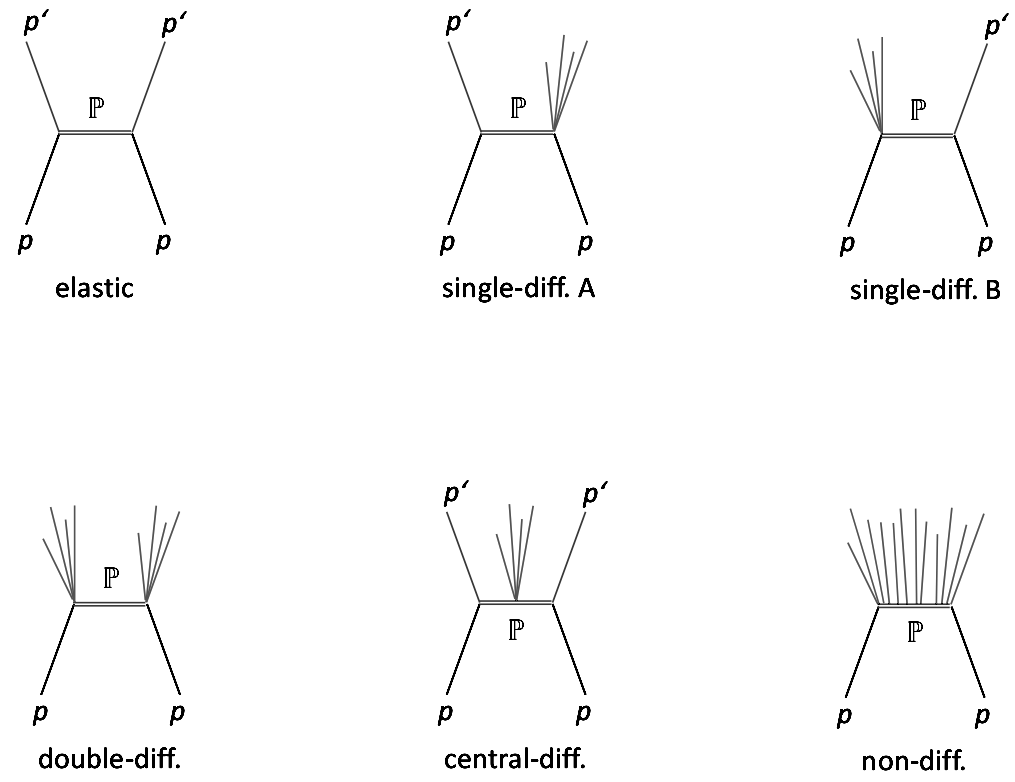
\includegraphics[width=13cm]{DiffractiveProzesse.png} 
\caption{Feynmann-Diagramme der möglichen Szenarien bei einer Proton-Proton-Kollision. Zeitachse hier von oben nach unten. Die durchgezogenen Linien, die in Zeitrichtung laufen, stellen den Verlauf der Protonen dar, während die Gruppierungen von Linien repräsentieren entstehende Teilchenstrahlen.}
\label{Diffractiv}
\end{figure}
Für die vorliegende Untersuchung werden noch weitere Auswahlkriterien für die Ereignisse angewendet. In der experimentellen Teilchenphysik drückt man den Winkel $\theta$ zwischen der Flugrichtung eines erzeugten Teilchens und der Strahlachse durch die sogenannte Pseudorapidität $\eta$ aus, die folgendemaßen im Zusammenhang mit dem erwähnten Winkel steht.\\
\begin{equation} \label{eq:Eta}
  \eta= -\ln{\tan{\dfrac{\theta}{2}}}
\end{equation}
Um die Qualität der Daten zu garantieren, wird in dieser Arbeit vorausgesetzt, dass der Polarwinkel $\theta$ mit der geometrischen Abdeckung der Detektoren TPC und ITS übereinstimmt. Daher erfordert man, dass die Pseudorapidität der gemessenen Teilchen sich im Intervall $|\eta| < 0.8$ befindet. Zu diesem selben Zweck wird daneben benötigt, dass nur Ereignisse berücksichtigt werden, deren Kollisionsvertices $V_{Z}$ innerhalb $\pm 10$ cm Abstand vom Nominalvertex ($V_{Z} = 0$) entlang der Stahlachse liegen. Die Abbildung ?? zeigt die Verteilung der Pseudorapidität $|\eta|$ sowie des Kollisionsvertex $V_{Z}$ der gemessenen Ereignisse.
\subsection{Spurselektion}
\label{sec:Spurselektion}
Im Rahmen dieser Arbeit werden unterschiedliche Auswahlkriterien für die Spuren der Teilchen angewendet, mit dem Ziel, lediglich die physikalisch relevanten Daten zu selektieren. Dabei sollte es betont werden, dass nur elektrisch geladene Teilchen können eine verfolgbare Spur hinterlassen. Teilchen, die entweder aus dem Zusammenprall oder aus Zerfälle entstehen, die in unmittelbarer Nähe des Kollisionsvertex vorkommen, und eine Lebensdauer $\tau > 1$ cm/c besitzen, die ihnen erlaubt, auf den Detektor zu treffen, nennt man im Kontext des ALICE-Experiments Primärteilchen. Diese Definition von Primärteilchen bezieht folgende Teilchen ein: Elektron $e^-$, Muon $\mu^-$, Pion $\pi^+$, Kaon $K^+$, Proton $p$, Xi-Baryon $\Xi^-$, Omega-Baryon $\Omega^-$ und die Sigma-Baryonen $\Sigma^+$ und $\Sigma^-$  sowie die entsprechenden Antiteilchen.\\
Im Wesentlichen bestehen die erwähnten Auswahlkriterien darin, die gemessenen Teilchenspuren, die eine geringe Qualität aufweisen, also die eine niedrige $p_{\mathrm{T}}$-Auflösung besitzen oder die keinen realen Spuren entsprechen, auszuschließen. Des Weiteren ist es darauf zu achten, dass die Detektoren nicht nur Primärteilchen messen, sondern auch diejenigen, die aus davon unabhängigen Prozesse stammen, wie andere Zerfälle, als die obengenannt wurden, oder Wechselwirkungen mit dem Detektormaterial. Solche Teilchen werden Sekundärteilchen genannt und sie müssen auch mittels Spurselektionen aus der Analyse verworfen werden.\\
Die erste Maßnahme in diese Richtung handelt sich darum, einen kinematischen Bereich $p_{\mathrm{T}} > 0.15$  $\mathrm{GeV}/c$ für die gemessenen Teilchen festzulegen. Außerdem bedient sich die in dieser Arbeit verwendete Analyse der in der Tabelle \ref{tab:Cuts} aufgelisteten Spurselektionen, die im Folgenden in Detail beschrieben werden.\\ \\
\begin{table}
\centering
\begin{tabular}{|c|c|c|}
\hline
\textbf{Id} & \textbf{Spurselektion} & \textbf{Voraussetzung} \\
\hline
1 & max. $\mathrm{DCA}_{z}$ & $2$cm\\
 &  & \\
\hline
2 & max. $\mathrm{DCA}_{xy}$ & $7\sigma$\\
 &  & \\
\hline
3 & max. Anteil von Spuren, die & $0.4$\\
& TPC-Cluster teilen & \\
\hline
4 & Auftreffen des Teilchens & benötigt\\
 & auf das SPD & \\
\hline
5 & max. Verhältnis von durchgequerten & $0.8$\\
  &  Reihen zu auffindbaren Clustern & \\
\hline
6 & geometrische Länge der Spur & $130$\\
 &  & \\
\hline
7 & geometrische Länge des & $3$cm\\
 & TPC-Ausschlussgebiets & \\
\hline
8 & max. $\chi^2$ per TPC-Cluster & $4$\\
 &  & \\
\hline
9 & max. $\chi^2$ per ITS-Cluster  & $36$\\
 &  & \\
\hline
10 & max. $\chi^2$ der in TPC  & $36$\\
 &  begrenzter Spur vs. globale Spur & \\
\hline
\end{tabular}
\caption{Auflistung der verwendeten Spurselektionen. Jeder Selektion wurde eine Identifikationsnummer zur Erleichterung ihrer Nennung zugewiesen.}
\label{tab:Cuts}
\end{table}
\textbf{Selektion der Primärteilchen}\\
Um zu gewährleisten, dass eine rekonstruierte Teilchenspur einem Primärteilchen entspricht, stellt man eine maximale Distanz vom Anfangspunkt der Spur zum Kollisionsvertex fest (englisch: \textit{Distance of closest approach to the vertex}, DCA abgekürzt). In Strahlrichtung, also in z-Richtung gemäß der Geometrie des ALICE-Detektors, erfordert man für jede Spur eine Distanz von $\mathrm{DCA}_{z} < 2$ cm, während in Radialrichtung eine von $\mathrm{DCA}_{xy} < 7\sigma$ benötigt wird, wobei $\sigma = 26 + \tfrac{50}{(p_{T}/\mathrm{GeV}/c)^{1.01}}$ die Standardabweichung der Stoßparameterauflösung bezeichnet. $\sigma$ dient dazu, die Fähigkeit des Detektors abzuschätzen.\\ \\
\textbf{TPC und ITS Selektion}\\
%Quelle:https://cds.cern.ch/record/2045797/files/Report.pdf
%Quelle: Phillip Luettig Master-Thesis
Zusätzlich zu den erwähnten Voraussetzungen für die DCA einer Spur verwendet man weitere Einstellungen (Selektionen 3 bis 10 in der Tabelle \ref{tab:Cuts}), die mit dem aus der TPC und dem ITS bestehenden Detektorsystem zusammenhängen:
\begin{itemize}
 \item Maximal $40\%$ der Cluster dürfen mehrere Spuren gleichzeitig teilen.
  \item Jede Spur muss erfüllen, dass das dazugehörige Teilchen auf die innerste Schicht des ITS, also auf das SPD, auftrifft. Dies vereinfacht den Ausschuss von Sekundärteilchen, die sich aus schwachen Zerfälle seltsamer Hadronen ergeben, denn solche Teilchen entstehen in der Regel zu einem späteren Zeitpunkt.
 \item Einige Reihen von Pads, die ein Teilchen in der TPC durchquert, können aufgrund der begrenzten Detektoreffizienz den Durchgang des Teilchens nicht aufzeichnen. Um die Anzahl von durchgequerten Reihen zu bestimmen, wird die Anzahl von Reihen, die zwar keine Spur detektieren, aber deren beiden benachbarten das Signal dafür senden, zur Anzahl von Clustern addiert. Darüber hinaus werden die Reihen, die wegen der Geometrie der Spur als mögliche Cluster bezeichnet werden können, auffindbare Cluster genannt. In dieser Analyse wird das Verhältnis von durchgequerten Reihen zu auffindbaren Clustern auf $80\%$ begrenzt.
 \item Ferner wird eine minimale Länge für die Teilchenspuren verlangt. In dieser Arbeit muss eine Spur mindestens $130$ Reihen von Pads durchqueren, um akzeptiert zu werden.
 \item Zusätzlich werden alle Pads in der TPC, die sich in einem Abstand von $3$ cm vom Rand des Detektors befinden, ausgeschlossen.
 \item Alle Spuren werden anhand von Bezugspunkte rekonstruiert, die das Teilchen in den verschiedenen Detektorschichten hinterlässt. Dafür werden diese Punkte so gefittet, dass man eine Kurve erhält, die die Teilchenbahn möglichst ähnlich beschreibt. Mit Hilfe der statistischen Mathematik lässt sich ein Maß für die Abweichung der einzelnen Bezugspunkte in den ITS- und TPC-Detektoren von dem globalen Fit definieren, den sogenannten $\chi^2$-Test (Chi-Quadrat-Test ausgesprochen). Je größer der Wert für das $\chi^2$ einer Spur beträgt, desto schlechtere Qualität diese Spur besitzt. In dieser Arbeit ist es bei $\tfrac{\chi^2}{cluster} < 4$ für die TPC und bei $\tfrac{\chi^2}{cluster} < 36$ für das ITS limitiert.
 \item Die Abweichung der Spur, die aus den sich nur im TPC befindenden Bezugspunkte resultiert, von der globalen Spur muss $\chi^2 < 36$ betragen.
\end{itemize}

\section{Korrekturen}
\label{Korr}
Unter Anwendung der im letzten Unterkapitel diskutierten Selektionen erhält man das unkorrigierte $p_{\mathrm{T}}$-Spektrum, das sich aus dem Datensatz ?? ergibt. Man beachte, dass die Abbildung ?? das auf die Anzahl von Ereignisse $N_{E}$ normierte $p_{\mathrm{T}}$-Spektrum illustriert und dass auf beiden Achsen zu einer übersichtlicheren Darstellung logarithmische Skala verwendet wurde.\\
%\begin{figure}
%\centering
%\includegraphics[width=10cm]{} 
%\caption{Kopplungskonstante der starken Wechselwirkung in Abhängigkeit des Abstands bzw. des Impulsüberträgs.}
%\label{RawSpectrum}
%\end{figure}
Diese Verteilung stellt die normierte Anzahl von Spuren, die in einem bestimmten $p_{\mathrm{T}}$-Intervall enthalten sind, dar. Zusätzlich steht diese selbe Verteilung zur Verfügung als Funktion von drei weiteren kinematischen Variablen, die die Spuren auch charakterisieren: die Pseudorapidität $\eta$, der Kollisionsvertex $V_{Z}$ und die Anzahl geladener Teilchen, auch Multiplizität genannt.\\
Trotzdem muss man berücksichtigen, dass die limitierte Detektoreffizienz, die begrenzte räumliche Abdeckung des Detektors, auch unter dem Name Akzeptanz bekannt, sowie die Kontamination durch Sekundärteilchen einen signifikanten Einfluss auf die Ergebnisse besitzen. Diese Tatsache verpflichtet der in der vorliegenden Arbeit präsentierten Analyse, das $p_{\mathrm{T}}$-Spektrum zu korrigieren. Wie im Abschnitt \ref{sec:MC} dargelegt, werden diese Korrekturen mithilfe von Monte-Carlo-Simulationen bestimmt. Für diese Arbeit werden die Monte-Carlo-Produktionen verwendet, die das ALICE-Experiment anbietet. Die Monte-Carlo-Periode, die die Korrektur der Datenperioden LHC17pq übernimmt, heißt LHC17l3b\_?? und sie wurde mit dem Monte-Carlo-Generator GEANT3 erzeugt.\\
%GEANT3 und PYTHIA--> Erklären!
In dieser Arbeit unterscheidet man hauptsächlich die Korrekturen danach, ob sie die Spuren oder die Ereignisse betreffen. Die Korrekturen der ersten Kategorie beeinflussen auf die Form des $p_{\mathrm{T}}$-Spektrums und sie können eine Abhängigkeit von dem Transversalimpuls $p_{\mathrm{T}}$ zeigen, während die von der zweiten Kategorie nur die Normierung der Verteilung beeinträchtigen. In dem zweiten Fall bleibt die Form des $p_{\mathrm{T}}$-Spektrums daher erhalten. Im Folgenden wird näher die verschiedenen Korrekturen, die im Zuge dieser Arbeit angewendet werden, erläutert. 

\subsection{Nachweiseffizienz}
Das benutzte Detektorsystem kann aufgrund von den diskutierten Kapazitätsbeschränkungen sowie von der Akzeptanz geladene Spuren nur mit einer bestimmten Wahrscheinlichkeit nachweisen. So, zum Beispiel, kommt es gelegentlich vor, dass die Krümmung einer rekonstruierten Spur von der Krümmung der echten Spur abweicht. Die rekonstruierte Spur kann dann eventuell verworfen werden, weil sie die Selektionskriterien nicht erfüllt, obwohl die echte Spur den Anforderungen entspricht.\\
Dies impliziert die Existenz einer gewissen Nachweiseffizienz des Detektors $\epsilon_{N}$, die eine entsprechende Korrektur verlangt. Solche Effizienz hängt von den vier kinematischen Variablen einer geladenen Spur ab: dem Transversalimpuls $p_{\mathrm{T}}$, der Pseudorapidität $\eta$, dem Kollisionsvertex $V_{Z}$ und der Multiplizität $M$. Die von den Monte-Carlo-Simulationen gelieferten Informationen werden dann verwendet, um das Verhältnis von rekonstruierten Spuren zu generierten Primärteilchen zu berechnen, aus dem sich die Nachweiseffizienz $\epsilon_{N}$ ergibt:
\begin{equation} \label{eq:TrackingEff}
  \epsilon_{N}=\dfrac{N^{MC}_{prim,rek}(p_{\mathrm{T}}, \eta, V_{Z}, M)}{N^{MC}_{prim,gen}(p_{\mathrm{T}}, \eta, V_{Z}, M)}
\end{equation}
In der Abbildung \ref{TrackingEff} ist die in der präsentierten Analyse erhaltene Nachweiseffizienz als Funktion des Transversalimpulses $p_{\mathrm{T}}$ ersichtlich. Insgesamt beobachtet man, dass die Nachweiseffizienz in einem Bereich zwischen $50$\% und  $80$\% bleibt. Es fällt auch auf, dass die Kurve bei niedrigem $p_{\mathrm{T}}$, d.h. zwischen $0.15 \mathrm{GeV}/c$ und $0.3 \mathrm{GeV}/c$, eine steigende Tendenz erfährt. Erklären lässt sich dieses Wachstum mit der starken Krümmung, die die Spuren wegen des magnetischen Feldes sowie des Energieverlustes bei dem Durchlauf durch das Material bei diesem konkreten $p_{\mathrm{T}}$-Intervall aufweisen. Dieses Phänomen erleichtert den Nachweis des Teilchens und es bewirkt somit den Anstieg bei der Effizienz.\footnote{nicht sicher, ob das stimmt. Perezs Thesis und Gronefelds widersprechen sich an dieser Stelle (Seiten 53 und 46). Frag Patrick!}. Bei rund $p_{\mathrm{T}} \thickapprox 1 \mathrm{GeV}/c$ beobachtet man allerdings eine bemerkenswerte Abnahme der Nachweiseffizienz, welche durch das Kriterium verursacht wird, dass die Spuren eine minimale geometrische Länge besitzen müssen (siehe Tabelle \ref{tab:Cuts}). Da die sich in diesem $p_{\mathrm{T}}$-Bereich befindenden Primärteilchen dazu neigen, die TPC durch die Ränder zu durchqueren, werden die jeweiligen Spuren durch das erwähnte Kriterium ausgeschlossen. Dies führt zu einer wenig effektiven Rekonstruktion der Spuren. Letztendlich erreicht die Nachweiseffizienz mit steigendem $p_{\mathrm{T}}$ und nach einer progressiven Zunahme ein Plateau von rund $70\%$.
%Quelle: Tesis de Edgar
%\begin{figure}
%\centering
%\includegraphics[width=5cm]{TrackingEff.png}  
%\caption{Nachweiseffizienz in Abhängigkeit von dem $p_{\mathrm{T}}$ geladener Teilchen in simulierten %pp-Kollisionen mithilfe von PYTHIA und GEANT3.}
%\label{TrackingEff}
%\end{figure}
\subsection{$p_{\mathrm{T}}$-Auflösung}
Der Transversalimpuls $p_{\mathrm{T}}$ geladener Teilchen wird anhand der Messung der Krümmung der entsprechenden Spuren berechnet. Solche Messung erfolgt durch eine bestimmte Ungenauigkeit, die mit steigendem $p_{\mathrm{T}}$ größer wird, denn die Krümmung der Spur wird parallel dazu immer unklarer. Dies zwingt zu einer Korrektur der $p_{\mathrm{T}}$-Auflösung.\\
Wie schon im Abschnitt \ref{sec:ALICE} erläutert, verwendet man den Kalman-Filter, um die im ITS und in der TPC vorhandenen Punkte eines fliegenden Teilchens zu fitten und dadurch die dazugehörige Spur zu gewinnen. Dabei stellt dieser Algorithmus verschiedene Variablen sowie die jeweiligen Fehler zur Verfügung, die die Spur in Form einer Matrix, die Kovarianzmatrix, parametrisieren. Der Kehrwert des Transversalimpulses $1/p_{\mathrm{T}}$ handelt sich um einen dieser Parameter. Die gesuchte relative $p_{\mathrm{T}}$-Auflösung $\sigma(p_{\mathrm{T}})/p_{\mathrm{T}}$ lässt sich wie folgt bestimmen:
\begin{equation} \label{eq:RelativePtResolution}
  \dfrac{\sigma(p_{\mathrm{T}})}{p_{\mathrm{T}}} \approx p_{\mathrm{T}} \cdot \sigma(1/p_{\mathrm{T}})= p_{\mathrm{T}} \cdot \sqrt{Cov(1/p_{\mathrm{T}}, 1/p_{\mathrm{T}})}
\end{equation}
%\begin{figure}
%\centering
%\includegraphics[width=5cm]{RelativePtResolution.png}  
%\caption{Relative $p_{\mathrm{T}}$-Auflösung als Funktion des Transversalimpulses.}
%\label{RelativePtResolution}
%\end{figure}
Aus dem analysierten Datensatz ergibt sich die in der Abbildung \ref{RelativePtResolution} gezeigte relative $p_{\mathrm{T}}$-Auflösung als Funktion des Transversalimpulses. Bei $p_{\mathrm{T}} \thickapprox 1 \mathrm{GeV}/c$ findet sich das Minimum dieser Funktion, welch $\sigma(p_{\mathrm{T}})/p_{\mathrm{T}} \thickapprox 1\%$ beträgt. Dieser Punkt bezeichnet die bestmögliche Auflösung im gesamten $p_{\mathrm{T}}$-Bereich. Bei größeren $p_{\mathrm{T}}$ verschlechtert sich die Auflösung und sie erreicht für $p_{\mathrm{T}}=150 \mathrm{GeV}/c$ den Wert $3.5 \%$.
%siehe Seite 63(Efgar) und Seite 54 (Julius) um den Einbau dieser Korrektur zu beschreiben
\subsection{Abschätzung der Sekundärteilchen}
%Quellen: Edgar, Julius, MKnichel Thesis. Analysis Note pp
Die im Unterkapitel \ref{sec:Spurselektion} beschriebenen Spurselektionen zielen unter anderem darauf ab, die Kontamination der gemessenen Daten durch Sekundärteilchen zu entfernen. Trotzdem bleibt ein Anteil, welcher zwar klein, aber signifikant ist, immer übrig. Dies fordert die Anwendung eine Korrektur, die diesen Anteil aus den Daten abzieht.\\
Wie schon angesprochen, werden den Sekundärteilchen Teilchen zugeordnet, die nicht unmittelbar mit der Kollision zusammenhängen, sondern die aus schwachen Zerfälle stammen, wie. z.B. aus Zerfälle von neutralen Kaonen $K^{0}$, von Lambda-Baryonen $\Lambda$ oder seltener von Myonen $\mu$. Neben solchen Fälle sind auch Teilchen, die aus Wechselwirkungen mit dem Detektormaterial resultieren, als sekundär definiert.\\
Zur Bestimmung des Anteils von Sekundärteilchen bedient man sich den $\mathrm{DCA}_{xy}$-Verteilungen, für die die gemessenen Daten und die Monte-Carlo-Simulationen sorgen. Das ist darauf zurückzuführen, dass die $\mathrm{DCA}_{xy}$ eines Primärteilchens sich von der eines Sekundärteilchens substantiell unterscheidet, denn der Ursprungspunkt der Teilchen der zweiten Gruppe befindet sich weiter von dem Kollisionsvertex. Es ist also erwartet, dass die jeweiligen $\mathrm{DCA}_{xy}$-Verteilungen verschiedenen Formen beschreiben. Dieser Unterschied wird besonders sichtlich an den Enden der Verteilungen.\\
Um allerdings die gesamte $\mathrm{DCA}_{xy}$-Verteilungen darstellen zu können, muss eine modifizierte Spurselektion angewendet werden. Die Selektionen $1$ und $2$ der Tabelle \ref{tab:Cuts} müssen deaktiviert werden, da sie die $\mathrm{DCA}_{xy}$-Verteilungen direkt betreffen. Für diesen selben Zweck wird auch auf die Selektion $10$ verzichtet. Trotzdem muss man berücksichtigen, dass diese Änderungen an der Spurselektion die Funktionalität des ITS beeinträchtigen, welche neben anderen darin besteht, \textit{pile up} Ereignisse von der Messung auszuschließen. Als alternative Methode zum Ausschuss solcher Ereignisse wird die TOF verwendet.\\
Mit den Messdaten verfügt man über die $\mathrm{DCA}_{xy}$-Verteilung der gemessenen Teilchen, ohne zu unterscheiden, ob es sich um Primär- oder Sekundärteilchen handelt. Der vorhandene Bruchteil von Sekundärteilchen wird abgeschätzt, indem man unter Einsatz eines computergesteuerten Verfahrens diese Verteilung anhand einer linearen Kombination der mit den Monte-Carlo-Simulationen erhaltenen Verteilungen, die sogenannten \textit{templates}, fittet. Die Monte-Carlo-Simulation bietet eine $\mathrm{DCA}_{xy}$-Verteilung der Primärteilchen und eine der Sekundärteilchen an.\\
Alle diese $\mathrm{DCA}_{xy}$-Verteilungen werden in drei verschiedenen $p_{\mathrm{T}}$-Bereiche dargestellt: $0.1 < p_{\mathrm{T}} < 0.5$ $\mathrm{GeV}/c$, $0.5 < p_{\mathrm{T}} < 1.0$ $\mathrm{GeV}/c$ und $1.0 < p_{\mathrm{T}} < 1.5$ $\mathrm{GeV}/c$. Die Analyse dieser $p_{\mathrm{T}}$-Intervalle genügt, um vorherzusagen, wie die Verteilung sich im gesamten $p_{\mathrm{T}}$-Bereich verhält. In der Abbildung \ref{RelativePtResolution} sind die $\mathrm{DCA}_{xy}$-Verteilungen für diese drei Bereiche gezeigt. Die aus den Messdaten resultierende Kurve liegt oberhalb der den Primärteilchen entsprechenden Verteilung, die sich wiederum oberhalb der Verteilung für die Sekundärteilchen befindet. In allen Fällen lässt sich eine deutliche Anhäufung von Ereignisse bei $\mathrm{DCA}_{xy} \approx 0 \mathrm{cm}$, also bei der Umgebung des Nominalvertex. Außerdem lässt sich die erwähnten Unterschiede in der Form der Diagramme beobachten. Insbesondere kann man erkennen, dass die Kurve der Sekundärteilchen eine breitere Anhäufung im Vergleich zu den anderen aufweist. Das bestätigt, dass die Ereignisse solcher Kurve nach Definition weiter von dem Nominalvertex vorkommen. Die Abbildung \ref{RelativePtResolution} zeigt auch das Verhältnis von der Fit-Funktion zu der $\mathrm{DCA}_{xy}$-Verteilung der Messdaten. Schließlich wird in der Abbildung \ref{ResultsFractionsDCA} die gesuchten Anteile von Primärteilchen (rot) bzw. Sekundärteilchen (grün) in den drei $p_{\mathrm{T}}$-Bereiche gezeichnet. Dabei stellen die farbigen Symbolen die sich aus den Daten ergebenden Anteile dar, während die leeren Symbolen aus den Monte-Carlo-Simulationen stammen. Die gewünschte Korrektur des $p_{\mathrm{T}}$-Spektrums lässt sich aus dem Verhältnis von den Anteile der Daten zu den der Simulationen bestimmen.
%\begin{figure}
%\centering
%\includegraphics[width=5cm]{DCAVerteilungen.png}  
%\caption{\textbf{oben}: $\mathrm{DCA}_{xy}$-Verteilungen im $p_{\mathrm{T}}$-Bereich $0.15 \mathrm{GeV}/c < p_{\mathrm{T}} < 0.5 \mathrm{GeV}/c$. Auf die y-Achse ist die Anzahl von Ereignisse aufgeführt, während die $\mathrm{DCA}_{xy}$ in $\mathrm{cm}$ auf die x-Achse angegeben ist.}
%\label{RelativePtResolution}
%\end{figure}

%\begin{figure}
%\centering
%\includegraphics[width=5cm]{ResultsFractionsDCA.png}  
%\caption{Anteile der Primärteilchen bzw. der Sekundärteilchen für die genannten p_{\mathrm{T}}-Bereiche. }
%\label{ResultsFractionsDCA}
%\end{figure}
\subsection{Triggereffizienz}
Der in der vorliegenden Arbeit verwendete Minimum Bias Trigger wirkt mit einer gewissen Effizienz, die Triggereffizienz $\epsilon_{T}$. Das bedeutet, dass er häufig die Art einer Kollision falsch beurteilt. Zum Beispiel kann er eventuell ein Ereignis als nicht-einfach diffraktiven Prozess aufzeichnen, wenn es in der Tat um einen einfach diffraktiven Prozess oder sogar um einen elastischen Stoß handelt. Dies verpflichtet der präsentierten Analyse, das $p_{\mathrm{T}}$-Spektrum entsprechend zu korrigieren. Solche Korrektur hängt mit den Ereignisse zusammen und sie besitzt somit keinen Effekt auf die Form der $p_{\mathrm{T}}$-Verteilung. Der Wert für Triggereffizienz wird dafür benutzt, das $p_{\mathrm{T}}$-Spektrum zu normieren.\\
Die Triggereffizienz $\epsilon_{T}$ kann zwar mithilfe der Monte-Carlo-Simulationen berechnet werden, aber sie lässt sich auch direkt aus dem Datensatz bestimmen. Die zweite Variante liefert einen akkurateren Wert als die erste. Für die Berechnung der Vertex- und Triggereffizienz $\epsilon_{T}$ wird folgende Formel angewendet:\\
\begin{equation}
\epsilon_{T}=\dfrac{N_{E, V_{Z}<10\mathrm{cm}}}{N_{E, \mathrm{Rekon}}}
\end{equation}
Dabei bezeichnet $N_{E, V_{Z}<10\mathrm{cm}}	$ die Anzahl von Ereignisse, deren Kollisionsvertices sich in einem Abstand kleiner als $10\mathrm{cm}$ vom Nominalvertex $V_{Z} = 0$ entlang der Kollisionsachse befinden. Andererseits stellt $N_{E, \mathrm{Rekon}}$ die Anzahl von rekonstruierten Ereignisse dar. Damit erhält man mittels dieser einfachen Rechnung ein präzises Maß für die Anzahl von physkalisch relevanten Ereignisse, die rekonstruiert wurden. In der Tabelle \ref{tab:Trigger} sind die resultierenden Triggereffizienzen für die betrachteten Datensätze zusammengefasst.
\begin{table}
\centering
\begin{tabular}{|c||c|}
\hline
\textbf{Datenmenge} & \textbf{Triggereffizienz  $\epsilon_{T}$} \\
\hline
\hline
CENT mit SDD & $100\%$  \\ 
\hline
CENT ohne SDD & $100\%$ \\ 
\hline
\end{tabular}
\caption{Vertex- und Triggereffizienzen $\epsilon_{T}$ in Prozent für die Datensätze CENT mit und ohne SDD.}
\label{tab:Trigger}
\end{table} 
\section{Systematische Unsicherheiten}
\begin{table}
\centering
\begin{tabular}{|c|c|c|c|c|}
\hline
\multicolumn{1}{|c|}{\textbf{Id}} & \multicolumn{1}{|c|}{\textbf{Spurselektion}} & \multicolumn{1}{|c|}{\textbf{Nominalwerte}} & \multicolumn{2}{|c|}{\textbf{Variationen}}\\
\hline
1 & max. $\mathrm{DCA}_{z}$ & $2 \mathrm{cm}$ & $1 \mathrm{cm}$ & $5 \mathrm{cm}$\\
 & & & &\\
\hline
2 & max. $\mathrm{DCA}_{xy}$ & $7\sigma$ & $4\sigma$ & $10\sigma$\\
 & & & &\\
\hline
3 & max. Anteil von Spuren, die & $0.4$ & $0.2$ & $1.0$\\
& TPC-Cluster teilen & & &\\
\hline
4 & Auftreffen des Teilchens & benötigt & \multicolumn{2}{|c|}{nicht benötigt}\\
 & auf das SPD & & \multicolumn{2}{|c|}{ }\\
\hline
5 & max. Verhältnis von durchgequerten & $0.8$ & $0.7$ & $0.9$\\
  &  Reihen zu auffindbaren Clustern & & &\\
\hline
6 & geometrische Länge der Spur & $130$ & $120$ & $140$\\
 &  & & &\\
\hline
7 & geometrische Länge des & $2 \mathrm{cm}$ & $2 \mathrm{cm}$ & $4 \mathrm{cm}$\\
 & TPC-Ausschlussgebiets & & &\\
\hline
8 & max. $\chi^2$ per TPC-Cluster & $4$ & $3$ & $5$\\
 &  & & & \\
\hline
9 & max. $\chi^2$ per ITS-Cluster  & $36$ & $25$ & $49$\\
 &  & & &\\
\hline
10 & max. $\chi^2$ der in TPC  & $36$ & $25$ & $49$\\
 &  begrenzter Spur vs. globale Spur & & &\\
\hline
\end{tabular}
\caption{Zusammenfassung der durchgeführten Variationen der Spurselektionen.}
\label{tab:SysUnsich}
\end{table}
Der vorliegende Abschnitt dient dem Zweck, die Quellen der systematischen Unsicherheiten präsentierter Analyse zu beschreiben und ferner diese selben Unsicherheiten auszuwerten.\\
In dieser Arbeit werden die Auswahlkriterien für die Spuren sowie für die Ereignisse als verantwortlich für die systematischen Unsicherheiten betrachtet. Jede dieses Auswahlkriterium trägt dazu vollkommen unabhängig von den anderen Kriterien bei. Aus diesem Grund ergibt sich der gesamte Wert systematischer Unsicherheiten aus der quadratischen Summe der einzelnen Beiträge:
\begin{equation}
\sigma_{sys, ges} = \sqrt{\sum_{i}{\sigma_{sys, i}}^2}
\end{equation}
Um die jeweiligen Beiträge auszurechnen, werden zuerst die in der Tabelle \ref{tab:Cuts} vorhandenen Werte einzeln innerhalb eines physikalisch sinnvollen Bereich variiert, wie die Tabelle \ref{tab:CutsVariation} zeigt. Anschließend wird für jede Variation das entsprechende korrigierte $p_{\mathrm{T}}$-Spektrum gezeichnet, ohne die anderen Selektionen zu modifizieren. In diesem Rahmen muss man begreifen, dass man über solche Spektren in Form von Histogrammen verfügt, dessen Wertebereich in Intervallen eingeteilt sind, die \textit{bins} genannt werden. Da jeder Selektion zwei Variationen zugeordnet werden, untersucht man bei jedem \textit{bin}, welches der beiden Spektren die größte Abweichung von dem Standardspektrum zeigt. Folglich erhält man die in der Abbildung \ref{SysUnsich} dargestellten Grafiken.	



\section{Ergebnisse}
Das am Anfang des Unterkapitels \ref{sec:Korr} vorgestellte $p_{\mathrm{T}}$-Spektrum beschreibt die Anzahl rekonstruierter Spuren, die sich in einem bestimmten $p_{\mathrm{T}}$-Bereich befinden und die eine gegebene Pseudorapidität $\eta$ besitzen. Solche Spuren erfüllen ferner bestimmte Selektionskriterien und sie stammen aus Ereignisse mit einem Kollisionsvertex, für den $V_{Z} < 10\mathrm{cm}$ gilt. Aufgrund von verschiedenen Effekte wie beispielsweise die begrenzte Detektoreffizienz oder die räumliche Akzeptanz muss es allerdings korrigiert werden. Die Implementierung der beschriebenen Korrekturen gibt als Ergebnis das korrigierte $p_{\mathrm{T}}$-Spektrum, welches sich wie folgt definieren lässt:
\begin{equation}
\begin{split}
N_\mathrm{corr}(p_{\mathrm{T}}, \eta) = N_{\mathrm{uncorr}}(p_{\mathrm{T}}) \\
\times C_{\epsilon_{N}}(p_{\mathrm{T}})  \times C_{Sec}(p_{\mathrm{T}}) \times C_{p_{\mathrm{T}}-Aufloesung}(p_{\mathrm{T}})
\end{split} 
\end{equation}
Dabei bezeichnet $C_{\epsilon_{N}}(p_{\mathrm{T}})$ die Korrektur im Bezug auf die Nachweiseffizienz, $C_{Sec}(p_{\mathrm{T}})$ die Korrektur zuständig für die Kontamination durch Sekundärteilchen und $C_{p_{\mathrm{T}}-Aufloesung}$ den Term, der die $p_{\mathrm{T}}$-Auflösung korrigiert.

\chapter{Zusammenfassung}
\chapter{Literaturverzeichnis}



\end{document}
